\documentclass{article}
\usepackage{graphicx}
\usepackage{amsmath}
\usepackage{tikz-cd}
\usepackage{adjustbox}
\usepackage{caption}
\usepackage{titling}
\usepackage{enumitem}
\usepackage{algorithm}
\usepackage{algpseudocode}
\usepackage{amssymb}
\usepackage{hyperref}
\usepackage{tikz}
\usetikzlibrary{automata,positioning}
\title{Principles Of Model Checking Exercises Solutions}

\newcommand{\cupdot}{\mathbin{\mathaccent\cdot\cup}}
\author{Dario Bekic}
\begin{document}
	
	\maketitle
	
	\section{Introduction}
	These are my solutions for the exercises of the book Principles Of Model Checking by Christel Baier and Joost-Pieter Katoen
	\section{3 Linear Time Properties}
	
	\subsection{Exercise 3.1}
	This is like giving a regular grammar.
	
	\begin{align*}
		&S \rightarrow aS' | \emptyset S''\\
		&S' \rightarrow aS'''|b'''|\\
		&S'' \rightarrow aS'''|b'''\\
		&S''' \rightarrow aS'
	\end{align*}
	
	\subsection*{Exercise 3.2}

	\begin{enumerate}[label=\alph*)]
		\item $f: TS \mapsto TS^*$ (set $TS$ of transitions systems with terminal states and $TS^*$ is the one without). $f(S, Act, \rightarrow, I, AP, L, F) = (S\sqcup \{s_f\}, Act, \rightarrow \cup \{ (t, \tau, s_f) | t \in F \}, I \setminus F, AP, L \cup \{(s_f, \emptyset)\})$ by viewing everything as a set.
		\item Suppose $\sigma \in Traces(TS^*_1) \land \sigma \notin Traces(TS^*_2)$. Let $\pi_1$ be a $TS_1^*$ path such that $Trace(\pi_1)=\sigma$. Either $\exists q. \pi_q=s_f$ or not. Assume the first case, and let $j$ be the index of the first element in $\pi_1$ such that $\pi_1 \neq s_f$. The path fragment $\pi'_1=\pi_{1,1},...,\pi_{1,j}$  is a maximal path in $TS_1$ since $\pi_{1,j}$ is a terminal state by construction. By hypothesis there must exist a path $\pi'_2 \in TS_2$ such that $Trace(\pi'_1)=Trace(\pi'_2)$ thus also $\pi_2'$ must be a maximal initial finite fragment path i.e. must end in a terminal state of $TS_2$. Now we can extend the path $\pi_2'$ with infinite loops and since $s_{fin}$ i.e. the phantom state added to $TS_2^*$ has no atomic proposition its trace will be equal to that of $\pi_1$. Namely, $\sigma= Trace(\pi_1)=Trace(\pi'_1)=Trace(\pi'_2)=Trace(\pi_2)$, contradicting the claim that $\sigma \notin Traces(TS_2^*)$.
	\end{enumerate}
	
	\subsection*{Exercise 3.3}
	
	\begin{algorithm}
		\caption{BFS for Invariant Checking (shortest counterexample)}
		\begin{algorithmic}[1]
			\Procedure{BFSInvariant}{$TS(S, Act, \rightarrow, I, AP, L), \phi$}
			\State $Q \gets \text{emptyQueue}()$
			\State $pred \gets \text{emptyMap}()$ \Comment{$pred[s]$ is predecessor of $s$; absent means unseen}
			\ForAll{$s \in I$}
			\If{$L(s) \not\models \phi$}
			\State \Return $\langle \textbf{false}, [s] \rangle$
			\EndIf
			\State $Q.\text{enqueue}(s)$
			\State $pred[s] \gets \bot$ \Comment{mark as seen; $\bot$ denotes start of path}
			\EndFor
			\While{$\neg Q.\text{empty}()$}
			\State $u \gets Q.\text{dequeue}()$
			\ForAll{$v \in post(u)$}
			\If{$v \notin \text{keys}(pred)$} \Comment{first time seen $\Rightarrow$ shortest}
			\State $pred[v] \gets u$
			\If{$L(v) \not\models \phi$}
			\State \Return $\langle \textbf{false}, \textsc{Reconstruct}(pred, v) \rangle$
			\EndIf
			\State $Q.\text{enqueue}(v)$
			\EndIf
			\EndFor
			\EndWhile
			\State \Return $\langle \textbf{true}, \text{emptyList} \rangle$ \Comment{invariant holds on all reachable states}
			\EndProcedure
			\Procedure{Reconstruct}{$pred, t$}
			\State $path \gets \text{emptyList}$
			\State $x \gets t$
			\While{$x \ne \bot$}
			\State $path.\text{append}(x)$
			\State $x \gets pred[x]$
			\EndWhile
			\State \Return $\text{reverse}(path)$
			\EndProcedure
		\end{algorithmic}
	\end{algorithm}
	
	\subsection*{Exercise 3.4}
	
	\begin{enumerate}[label=\alph*)]
		\item $\implies$: pick a finite path fragment $\pi \in PathFragment_{fin}(TS)$ such that $Trace(\pi) \in Traces_{fin}(TS) \land Trace(\pi) \notin Traces_{fin}(TS')$. Call $\sigma$ the size of $\pi$. I can extend $\pi$ to a maximal path $\pi'$ such that $Trace(\pi') \in Traces(TS) \land Trace(\pi') \in Traces(TS')$. By $Trace(\pi') \in Traces(TS')$ there must exist a path $\rho' \in Paths(TS')$ such that $Trace(\rho') = Trace(\pi')$. Thus, the prefix of length $\sigma$ of $\rho'$ is a finite path fragment $\rho$ in $TS'$ such that $Trace(\rho)=Trace(\pi)$, contradicting the hypothesis $Traces(\pi) \notin Traces_{fin}(TS')$. The same can be argued by swapping $TS$ and $TS'$ roles, completing the proof.\\
		$\impliedby$: pick a path $\xi \in Paths(TS)$ such that $Trace(\xi) \in Traces(TS) \land Trace(\xi) \notin Traces(TS')$. I argue that for any $n \in \mathbb{N}$ there exists a path fragment $p^n$ in $TS'$ such that its trace its equal to the prefix of length $n$ of $\xi$ and that it can be extended to path fragment of size $n+1$ which is equal to the trace of the prefix of length $n+1$ of $\xi$. 
		The first part of the statement comes directly from the assumption that the finite traces sets equal each other. The second part comes from the fact any trace in both transition systems can be given by only one path (or path fragment), thus for the prefix of length $n+1$ of $\xi$ i need necessarily to extend $p^n$ because if there was another path different from $p^n$, call it $p^*$, then their prefix trace of size $n$ would be the same, contradicting the claim.
		Suppose that in fact such $p^*$ existed, then it may share a prefix of states with $p^n$, let $q < n$ be the last state they share, i.e. $p^*_q = p^n_q$ then there should be two states $p^*_{q+1}$ and $p^n_{q+1}$ such that $L(p^*_{q+1})=L(p^n_{q+1})$ because $p^*, p^n$ share the same trace up to the first $n$ states, but this contradicts AP determinism.
		\item 
		\begin{tikzcd}
			{} \arrow[rd] &                                                   & {} \arrow[rd]   &                                                                            &                 &                 &      \\
			& \{x\} \arrow[loop, distance=2em, in=305, out=235] &                 & \{x\} \arrow[lld] \arrow[d] \arrow[rd] \arrow[rrd] \arrow[ld] \arrow[rrrd] &                 &                 &      \\
			& \{x\}                                             & \{x\} \arrow[l] & \{x\} \arrow[l]                                                            & \{x\} \arrow[l] & \{x\} \arrow[l] & ....
		\end{tikzcd}
	\end{enumerate}
	\subsection*{Exercise 3.5}
	\begin{enumerate}[label=\alph*)]
		\item $\verb|false| \triangleq \emptyset$
		\item $\verb|initEqualZero| \triangleq \{A_0A_1,... \in (2^{AP})^\omega | \exists i \in \mathbb{N}. A_i = \{x=0\} \land \forall j < i. A_j = \emptyset \}$
		\item $\verb|initDiffZero| \triangleq (2^{AP})^\omega \setminus \verb|initEqualZero|$
		\item This seems not to be safety nor liveness.
		\item Liveness property
		\item Liveness property
		\item $\verb|initEqualZero| \triangleq \{A_0A_1,... \in (2^{AP})^\omega | (A_i = \{x=0\} \land A_{j} = \{x > 0\} \land \text{i even, j odd}) \lor (A_i = \{x=0\} \land A_{j} = \{x > 0\} \land \text{i odd, j even})\}$
		\item $\verb|true| \triangleq (2^{AP})^\omega$
	\end{enumerate}
	\subsection*{Exercise 3.6}
	\begin{enumerate}[label=\alph*)]
		\item Invariant: $\verb|Never| \triangleq \{A_0A_1,... \in (2^{AP})^\omega | A \notin A_i \forall i\}$
		\item Safety: $\verb|Once| \triangleq \{A_0A_1,... \in (2^{AP})^\omega | \exists i. A \in A_i \land \forall j. (j < i \lor j > i) \land A \notin A_j \}$
		\item Liveness: $\verb|AlternateInfinitely| \triangleq \{A_0A_1,... \in (2^{AP})^\omega | \exists i, j, q. j > i \land A_j = \{A\} \land q > i \land A_q = \{B\} \land (\forall t > i. A_t = \{A\} \implies \exists x. A_x = \{B\} \land \forall c . i < c < x. B \notin A_c) \land (\forall t > i. A_t = \{B\} \implies \exists x. A_x = \{A\} \land \forall c . i < c < x. A \notin A_c)\}$ (its a liveness property because the $i$ existential witness can be large as one wishes).
		\item Liveness $\verb|AlternateInfinitely| \triangleq \{A_0A_1,... \in (2^{AP})^\omega | \exists i. ((\exists j < i . A \in A_j \land \forall c. j < c < i. B \notin A_c) \implies B \in i) \land (\forall q. q > i \land (A \in A_q \implies \exists t. t > q. B \in A_t))\}$
	\end{enumerate}
	\subsection*{Exercise 3.7}
	Initial values: $r_1 = 0, r_2 = 1$.
	$y$ value is given by the value of register $r_2$ and the formula is $((r_1 \oplus x) \lor (x \land r_1))$.
	$r_1$ value is given by $(r_1 \oplus x) \lor (r_2 \land x)$
	
	\begin{enumerate}[label=\alph*)]
		\item Let $\alpha_{P_i}$ be a word in $P_i$ and $\beta_{P_i}$ be a word in $(2^{AP})^\omega \setminus P_i $.$\alpha_{P_1} \triangleq \{r_2, x, y\}(A)^\omega$ where $A \triangleq AP $,  $\alpha_{P_2} \triangleq \{r_1, x\} \cdot (\emptyset)^\omega$, $\alpha_{P_3} \triangleq (\{y\}, \emptyset)^{\omega}$, $\alpha_{P_4} \triangleq \emptyset^\omega$, $\beta_{P_1} \triangleq \{x\}^{\omega}$, $\beta_{P_2} \triangleq \{r_2, r_1\}^{\omega}$, $\beta_{P_3} \triangleq \{y\}^{\omega}$, $\beta_{P_4} \triangleq \{x, r_1\}^{\omega}$
		\item \begin{enumerate}[label=P\arabic*)]
			\item If $x=1$ is high will be high regardless of $r_1$: if $r_1=0$, $r_1 \oplus x$ will be 1, if $r_1=1$ then $x \land r_1$ will be 1. Thus it is satisfied.
			\item If $r_2 = 0, r_1 = 0$ in any state, in the next state we will $r_1=1$ if $x=1$ so it is not satisfied.
			\item This is not satisfied because $P_1$ is satisfied.
			\item False, it is a possible initial state
		\end{enumerate}
		\item P2, P3, P4 are safety properties and only P4 is an invariant.
		\begin{enumerate}[label=\roman*)]
			\item Let $X_i$ be equal to any set in $\{x, r_1, r_2, y\}$ of size i. $S^*$ is the terminal state of the grammar: with that symbol we can expand to any set of properties.
				\begin{enumerate}[label=P\arabic*), start = 2]
				\item \begin{align*}
					&S \rightarrow X_i \setminus \{r_2\} S' | X_i \cup \{r_2\} S\\
					&S' \rightarrow X_i S' | X_i \cup \{r_1\} S^* \\
				\end{align*}
				\item \begin{align*}
					&S \rightarrow X_i S | X_i \cup \{y\} S'\\
					&S' \rightarrow X_i \cup \{y\} S* \\
				\end{align*}
				\item \begin{align*}
					&S \rightarrow X_i S | X_i \cup \{x\} \setminus \{r_1\} S^*
				\end{align*}
			\end{enumerate}
		\item There is only $P4$: $\phi \triangleq \lnot x \lor r_1$
		\end{enumerate}
	\end{enumerate}
	\subsection*{Exercise 3.8}
	$\implies$: this direction holds and directly comes from the definition of closure of a property: $closure(P) = \{\alpha \in (2^{AP})^\omega | pref(\alpha) \subseteq pref(P) = \{\alpha \in (2^{AP})^\omega | pref(\alpha) \subseteq pref(P') = closure(P')\}$.\\
	$\impliedby$: suppose $closure(P) = closure(P')$ but $\alpha \in pref(P) \land \alpha \notin pref(P')$. Since $\alpha \in pref(P)$ there exists $\sigma \in P$ such that $\alpha$ is a prefix of $\sigma$. By definition of closure, $\sigma \in closure(P)$ which implies $\sigma \in closure(P')$ by hypothesis. But $\sigma \in closure(P') \iff pref(\sigma) \subseteq pref(P')$ by definition of closure, and thus we have $\alpha \in pref(P')$.
	\subsection*{Exercise 3.9}
	We need to show that i) the set $\Phi \triangleq closure(Traces(TS))$ is a LT  safety property and ii) that $TS$ satisfies it. 
	\begin{enumerate}[label=\roman*)]
		\item imagine there were $\alpha = A_0A_1,... \in (2^{AP})^{\omega} \setminus \Phi$ such that there exists $\pi \in pref(\alpha)$ such that $\Phi \cap \{\beta \in (2^{AP})^{\omega} | \pi \in pref(\beta)\} \neq \emptyset$. 
		Since $\alpha \notin closure(Traces(TS))$ it means there is a finite prefix of $\alpha$ that is not a prefix of some trace in TS. Let this trace be our $\pi$.
		Then if $\sigma \in \Phi \cap \{\beta \in (2^{AP})^{\omega} | \pi \in pref(\beta)\}$ it means $pref(\sigma) \subseteq pref(Traces(TS))$ which means $\pi \in pref(Traces(TS))$.
		\item A word $\xi$ is in $\Phi$ if and only if $pref(\xi) \subseteq pref(Traces(TS))$. Any path $\rho$ in TS has $Trace(\rho) \in Traces(TS)$ thus $pref(Trace(\rho)) \subseteq pref(Traces(TS))$.  
	\end{enumerate}
	\subsection*{Exercise 3.10}
	Suppose $\phi \in pref(closure(P))$ then $\exists \rho \in closure(P)$ such that a finite prefix of $\rho$ is $\phi$. But any element in $closure(P)$ is just a word whose prefixes are elements of $pref(P)$ thus any prefix of $\rho$ is a an element of $pref(P)$, even $\phi$, thus $\phi \in pref(P)$.
	\subsection*{Exercise 3.11}
	\begin{enumerate}[label=\alph*)]
		\item $\verb|UNION_SAFE| \triangleq P \cup P'$ is a safety property if $P, P'$ are safety properties. Consider $w \in \verb|UNION_SAFE|$. For it to be a safety property, it is sufficient to prove that for any $\rho \in (2^{AP})^\omega \setminus (\verb|UNION_SAFE|)$ and for any finite prefix $\pi$ of it $(\verb|UNION_SAFE|) \cap (\underbrace{\{\alpha \in (2^{AP})^\omega| \pi \text{ is a finite prefix of } \alpha\}}_{\triangleq \verb|PREFIX|})=\emptyset$.
		This equals to say, by distributivity, $(P \cap \verb|PREFIX|) \cup (P' \cap \verb|PREFIX|) = \emptyset$. Since $P, P'$ are safety properties we have $\emptyset \cup \emptyset = \emptyset$.
		\item $\verb|INTER_SAFE| \triangleq P \cap P'$ is a safety property if $P, P'$ are safety properties. Take any word $w \in (2^{AP})^\omega$. There are 2 cases to consider:
		\begin{enumerate}[label=\roman*)]
			\item $w \notin P \cup P'$: we wish to show  that for any finite prefix $\pi \in pref(w)$ , $P \cap P' \cap \underbrace{\{\alpha \in (2^{AP})^\omega | \pi \text { is a finite prefix of } \alpha\}}_{\triangleq \verb|PREFIX|}$. But since $P'$ is a safety property $P' \cap \verb|PREFIX|=\emptyset$, thus $P \cap \emptyset = \emptyset$.
			\item $w \in P' \land w \notin P$: we wish to show again that for any finite prefix $\pi \in pref(w)$ , $\verb|INTER_SAFE| \cap \verb|PREFIX| = \emptyset$. By commutativity of intersection, $P \cap P' \cap \verb|PREFIX| = P' \cap P \cap \verb|PREFIX| = P' \cap \emptyset = \emptyset$. The case of $w \in P \land w \notin P'$ is identical.
		\end{enumerate} 
	\item $\verb|UNION_LIVE| \triangleq P \cup P'$ is a liveness property if $P, P'$ are liveness properties. This is trivially arguable informally: if i can extend any finite prefix to a trace in $w_p \in P$ or to a trace $w'_{p} \in P'$ then i can extend any prefix to a trace in $P \cup P'$ (just pick either $w_p$ or $w_p'$).
	\item $\verb|INTER_LIVE| \triangleq P \cap P'$ is not necessarily a liveness property. To see a concrete counter-example consider $P\triangleq \{\text{ from one point there will be only 1s}\}$ and $P' \triangleq \{\text{ from one point there will be only 0s}\}$. Their intersection is empty, and the empty set is not a liveness property.		
	\end{enumerate}
	\subsection*{Exercise 3.12}
	\begin{enumerate}[label=\arabic*.]
		\item $closure(P) \subseteq P_{safe}$. Assume there exists $\alpha \in closure(P)$ such that $\alpha \notin P_{safe}$. Since $\alpha \in closure(P)$, for any finite prefix $\beta$ of $\alpha$, $\beta \in pref(\alpha) \implies \beta \in pref(P)$. So pick any prefix $\beta$ of $\alpha$, since $P_{safe}$ is a safety property we have $P_{safe} \cap \{\gamma | \beta \in pref(\gamma)\}=\emptyset$. But we also proved $\beta \in pref(P)$, and since $P$ contains a subset of $P_{safe}$ it means $\exists \lambda \in P_{safe}. \beta \in pref(\lambda)$. But this would imply $\lambda \in P_{safe} \cap \{\gamma | \beta \in pref(\gamma)\} \neq \emptyset$.
	\item $P_{live} \subseteq \underbrace{P \cup ((2^{AP})^\omega \setminus closure(P))}_{\verb|EXPR|}$. Suppose $w \in P_{live}$ but not in $\verb|EXPR|$. This can only happen if $w \notin P$ which implies $w \notin P_{safe}$. We wish to prove $w \in \verb|EXPR|$ if $w \notin P_{safe}$. This is equal to proving $w \notin P_{safe} \implies w \notin closure(P)$ by definition of $\verb|EXPR|$. We can prove the contrapositive: $w \in closure(P) \implies w \in P_{safe}$ which we proved in the first point.
	\end{enumerate}
	\subsection*{Exercise 3.13}
	One can of course use the Decomposition theorem, but there is a way of giving explicitly the two properties by using intuition.
	
	One would of course first start from characterizing $P$: maybe the exercise is tricky and $P$ is a safe or liveness property. Proving one such result would let us quickly end the exercise.
	
	\begin{enumerate}[label=\alph*.]
		\item Is $P$ a safety property? One could argue that the set of bad prefixes is $\{w_1,w_2,.. \in (2^{AP})^{\omega} | \exists n \in \mathbb{N}. w_n = \{a,b\} \land \exists j \in \mathbb{N}. j < n \land a \notin w_j\}$. However, the condition to have \textit{infinitely} many $j \in \mathbb{N}. b \in w_j$ cannot be captured by a finite prefix. In conclusion, $P$ is not a safety property.
		\item Is $P$ a liveness property? No, clearly $w'=\{\{b\}, \{a,b\}\}$ cannot be extended to a word satisfying $P$.
	\end{enumerate}
	
	Even though we were unsuccessful in proving safety or liveness, we identified the parts that were problematic during our proof attempt.
	
	In particular:
	$$
	P_{safe} \triangleq (2^{AP})^\omega \setminus  \{w_1,w_2,.. \in (2^{AP})^{\omega} | \exists n \in \mathbb{N}. (w_n = \{a,b\} \land \exists j \in \mathbb{N}. j < n \land a \notin w_j)\}
	$$
	and
	$$
	P_{live} \triangleq \{w_1,w_2,... | \overset{\infty}{\exists} j. b \in w_j\}
	$$
	The correctness is immediate.
	\subsection*{Exercise 3.14}
	First, let's put here the transition graphs.
	Consider the TS for Peterson's algorithm in \autoref{fig:peterson-transition-system} and for the Semaphore-based mutual exclusion in \autoref{fig:semaphore-transition-system}.
	Note that we have $req_1, req_2$ labels even though they are not in AP just for ease of read.
	In general we can solve this exercise by reasoning on the LT properties that the transition systems satisfy or not. As we know, the semaphore transition systems does not guarantee starvation freedom i.e. it is possible that one process will never enter its critical region.
	
	Thus, the trace:
	
	$$
	w \triangleq \{\{req_1, req_2\}, \{wait_1, req_2, \}, \{crit_1, req_2\}\}^{\omega}
	$$
	
	is in $Traces(TS_{sem})$ but not in $Traces(TS_{pet})$.
	\subsection*{Exercise 3.15}
	\begin{enumerate}[label=(\alph*)]
		\item Regarding satisfaction of $E'$: without \textit{unconditional} fairness assumptions it is a matter of verifying if there exists a path which contains $\{\{a\}, \{a,b\}, \emptyset\}$ and this is true $s_1 \rightarrow s_2 \rightarrow s_3 \rightarrow s_1$, thus this property is never satisfied.
		For $B_1$ only $E_a$ because we may loop on $s_1 \rightarrow s_2 \rightarrow s_1$. For $B_2$ both $E_a$ and $E_b$ as we need to exit the loop we mentioned because $s_1 \rightarrow s_3$ is infinitely enabled.
		For $B_3$ only $E_b$, because of the loops $s_1 \rightarrow s_2 \rightarrow s_1$ and $s_1 \rightarrow s_2 \rightarrow s_4 \rightarrow s_1$ we always pass by $s_1$ which has enabled the $\beta$ transition to $s_3$.
		\item The same reasoning for $E'$ applies. Now, recall that weaker assumptions restrict \textit{the same} or more traces, thus we do not check again those we proved are not satisfied by strong assumptions. For example, $B_1$ now looses $E_a$ as $\alpha$-transitions from $s_1$ are not continuously enabled, as we can loop on $s_1 \rightarrow s_3 \rightarrow s_1$. The same goes for $B_3$. And we also loose both $E_a, E_b$ for $B_2$ as we can loop on $s_1 \rightarrow s_2 \rightarrow s_1$ continuously \textit{alternating} between having $\alpha$ and $\beta$ transitions.
	\end{enumerate}
	\subsection*{Exercise 3.16}
	\begin{enumerate}[label=(\alph*)]
		\item 
		\begin{enumerate}[label=\arabic*.]
			\item With no assumption this is false. Let $AP_1 = \{\alpha\}$ and $AP_2=\{\beta\}$. Then let $\forall s \in S_2. \beta \in L(s), \forall s' \in S_1. \alpha \in L(s')$. Then $\forall A_1,A_2... \in Traces(TS_1 || TS_2)$ we have $\beta \in A_i$ but no trace in $TS_1$ contains such label (as it is not part of $TS_1$ label set).
			\item This is false. Consider \autoref{fig:ex3.16:a} where $\langle s_1, s_1'\rangle$ is the initial state and consider $Syn=\{\alpha\}$. It will be impossible to move out of the initial state as $s'_1$ has no outgoing $\alpha$ transition to synchronize on. We have only have one trace: $Traces(TS_1 || TS_2)=\{\{Trace(\langle s_1, s_1'\rangle)\}\}=\{\{L_1(s_1)\}\}$
			\begin{figure}[ht]
				\centering    
				\adjustbox{scale=1,center}{
					\begin{tikzcd}
						& s_1 \arrow[ld, "\alpha"] &                                                            & s'_1 \arrow[ld, "\beta"] \\
						s_2 \arrow["\alpha"', loop, distance=2em, in=305, out=235] &                          & s'_2 \arrow["\beta"', loop, distance=2em, in=305, out=235] &                         
				\end{tikzcd} }
				\caption{Exercise 3.16. point (a)}
				\label{fig:ex3.16:a}
			\end{figure}
		\end{enumerate}
		\item
		\begin{enumerate}[label=\arabic*.]
			\item With no assumption it is the same as (a).
			\item Assuming $AP_2 = \emptyset$ the result is true. Let us restrict to the subset of paths in $TS_1 || TS_2$ that use only a transition from $TS_1$. We argue that for any path $\sigma_1 = s_0,s_1,... \in Paths(TS_1)$ we have a path $\sigma_2 = \langle s'_0,s'_1,...\rangle$ such that $\pi_1(s'_i)=s_i$, where $\pi_1$ is the left projection. This can be proved easily by induction.
		\end{enumerate}
		\item 
		\begin{enumerate}[label=\arabic*.]
			\item With no assumption it is the same as (a).
			\item Assuming $AP=\emptyset$ it is still false. Consider \autoref{fig:ex3.16:c}. The transition system $TS_1 || TS_2$ allows for the path $P \triangleq (\langle s_1, s_1'\rangle \overset{\beta}{\rightarrow} \langle s_1, s_1'\rangle)^\omega$ with $Trace(P)=a^{\omega}$. However this trace is not available to $TS_1$ whose trace set is $\{\{a\cdot b^{\omega}\}\}$.
			\begin{figure}[ht]
				\centering    
				\adjustbox{scale=1,center}{
					\begin{tikzcd}
						& s_1\{a\} \arrow[ld, "\alpha"] &  & s'_1 \emptyset \arrow["\beta"', loop, distance=2em, in=305, out=235] \\
						s_2 \{b\} \arrow["\beta"', loop, distance=2em, in=305, out=235] &                               &  &                                                                     
						\end{tikzcd}}
				\caption{Exercise 3.16. point (c)}
				\label{fig:ex3.16:c}
			\end{figure}
			
		\end{enumerate}
		\item False. Consider \autoref{fig:ex3.16:d} and the two transition systems, where we just write the Atomic Propositions that hold:
		\begin{figure}[ht]
			\centering    
			\adjustbox{scale=1,center}{
						\begin{tikzcd}
					& \{a\} \arrow["\alpha"', loop, distance=2em, in=305, out=235] \arrow[ld, "\rho"] &       & \{a\} \arrow[ld, "\alpha"] \arrow["\rho"', loop, distance=2em, in=305, out=235] \\
					\{a\} &                                                                                 & \{a\} &                                                                                
					\end{tikzcd} }
			\caption{Exercise 3.16. point (d)}
			\label{fig:ex3.16:d}
		\end{figure}
		 and call the TS on the left $TS_1$ and the one on the right $TS_2$. It is obvious that $Traces(TS_1) \subseteq Traces(TS_2)$ as $Traces(TS_1) = Traces(TS_2)$.
		Clearly for $\mathcal{F}_{strong}=\{\{\alpha\}\}$ $TS_2$ has no infinite fair traces as it \textit{has} to take the $\alpha$ transition while $TS_1$ does.
		\item We simply make a little change to the transitions systems of the point (d). As you can see in figure 4., we have clearly $Traces(TS_1)=\{a^\omega\} \cup \{a^n\cdot b | n \in \mathbb{N}\}=Traces(TS_2)$ thus $Traces(TS_1)\subseteq Traces(TS_2)$.
		Consider the liveness property:
		$$
		\verb|EVENTUALLY_B| \triangleq \exists n. b \in A_n
		$$
		
		Under $\mathcal{F}=\{\emptyset, \{\{\alpha\}\}, \emptyset\}$ we have $TS_2 \models_{\mathcal{F}} \verb|EVENTUALLY_B|$ but $TS_1 \not \models_{\mathcal{F}} \verb|EVENTUALLY_B|$.
		\begin{figure}[ht]
			\centering
			\adjustbox{scale=1, center}{
		\begin{tikzcd}
			& \{a\} \arrow["\alpha"', loop, distance=2em, in=305, out=235] \arrow[ld, "\rho"] &       & \{a\} \arrow[ld, "\alpha"] \arrow["\rho"', loop, distance=2em, in=305, out=235] \\
			\{b\} &                                                                                 & \{b\} &                                                                                
		\end{tikzcd}}
		\caption{Exercise 3.16. point (e)}
		\end{figure}
	\end{enumerate}
	\subsection*{Exercise 3.17}
	It is enough to count all the cycles and see if one of those two non-mutually exclusive (but sufficient) conditions hold: $i)$ to access the cycle by using any path we encounter \textit{a} or $ii)$ in at least one state of the cycle we have available either a $\alpha$ or $\beta$ as outgoing transitions to states where \textit{a} holds (or where we have proved that it eventually holds).
	\\
	(Some) cycles are:
	\begin{enumerate}[label=\arabic*]
		\item $s_1 \rightarrow s_1$: since in $s_1$ \textit{a} holds we conclude by criterion $i)$.
		\item $s_2\rightarrow s_3 \rightarrow s_2$: we have infinitely many times $\beta$ transition available which sends us to $s_1$, thus by criterion $ii)$ and point 1. we conclude. 
		\item $s_3 \rightarrow s_4 \rightarrow s_5 \rightarrow s_4 \rightarrow s_6 \rightarrow s_3$ both criterion do not hold, thus the property is not satisfied.
	\end{enumerate}
	\subsection*{Exercise 3.18}
	\begin{enumerate}[label=(\alph*)]
		\item It is not realizable as there is no fair path starting from $s_1$ which is reachable with an $\alpha$ transition from $s_0$ because of the unconditional assumption $\{\alpha\}$.
		\item By having now the unconditional assumption $\{\delta, \alpha\}$ the loop $s_1 \rightarrow s_4 \rightarrow s_1$ is a fair path. Thus, $\mathcal{F}_2$ is realizable.
		\item This is too realizable. The loop $s_1 \rightarrow s_4 \rightarrow s_1$ will enable infinitely many times $\beta$ and by strong fairness $\{\alpha, \beta\}$ we will be forced to take it infinitely many times thus satisfying the unconditional assumption $\{\beta \}$.
	\end{enumerate}
	\subsection*{Exercise 3.19}
	\begin{enumerate}[label=(\alph*)]
		\item \begin{enumerate}[label=(\roman*)]
			\item
			\begin{align*}
			E 	&::= R_1(R_2^{\omega})\\
			R_1	&::= R'_1 | \epsilon\\
			R'_1 &::= \emptyset R'_1 | a\\
			R_2 &::= \{a\}R'_2 | \{b\}R_2 | \{a,b\}R_2\\
			R'_2 &::= \{b\}R_2
			\end{align*}
			\item
			By the decomposition theorem we have 
			\begin{align*}
			P_{safe}&=\{A_0A_1... \in (2^{AP})^{\omega} | ...\}\\
			...&=\exists n. (A_n =\{a\} \land \forall j. j < n \land A_j = \emptyset \land \forall k. k > n. A_k = \{a\} \implies A_{k+1} = \{b\} ) \cup \emptyset^{\omega}\\
			P_{live}&=P_1 \cup ((2^{AP})^\omega \setminus closure(P))\\
			&=(\{b\} + \{a,b\})^\omega \cup P_1 \cup \{A_0A_1... \in (2^{AP})^\omega | ...\} \cup \{\{a\}A_1... | *\}\\
			&...=\exists n.(n > 0 \land A_n = \{a\} \land \exists j < n. A_j \in \{\{a, b\}, \{b\}\} )\\
			&*=\exists i > 0. A_i = \{a\} \land A_{i+1} \neq \{b\}
			\end{align*}
			\item 
			\begin{enumerate}[label=\arabic*.]
				\item Suppose $w \in (2^{AP})^\omega \setminus P_{safe}$. If $\nexists i. w_i = \{a\}$ then pick $j$ the first non-empty set of $w$: it should be clear that any word with this prefix is not in $P_{safe}$. If $\exists i. w_i = \{a\}$ then it must be:
				\begin{enumerate}[label=\roman*.]
					\item Either $exists j. j < n \land A_j \neq \emptyset$. Then it is sufficient to pick the prefix $A_0...A_i$.
					\item Or(they are not mutually exclusive) $\exists k > i. A_{k} = \{a\} \land A_{k+1} \neq b$. Pick the prefix $A_0, ...A_{k+1}$.
				\end{enumerate}
			\end{enumerate}
		\end{enumerate}
		\item First, let's re-draw the transition system which we can see in \autoref{fig:ex3.19:b}, where each node is denoted with the pair $s \{L(s)\}$.
		\begin{figure}[ht]
			\centering
			\adjustbox{scale=1, center}{
					\begin{tikzcd}
						{} \arrow[rd] &                                                                                                                                          &  &                                                                                                             &  &                                                                    \\
						& s_0 \{a\}  \arrow[rr, "\alpha", bend left] \arrow[dd, "\beta"]                                                                 &  & s_1 \{b\} \arrow[ll, "\gamma", bend left] \arrow["\alpha" description, loop, distance=2em, in=125, out=55]  &  &                                                                    \\
						&                                                                                                                                          &  &                                                                                                             &  &                                                                    \\
						& {s_2\{a,b\}} \arrow["\alpha"', loop, distance=2em, in=305, out=235] \arrow[rr, "\delta"'] \arrow[rruu, "\gamma", bend right, shift left] &  & s_3 \emptyset \arrow[uu, "\alpha"] \arrow[rr, "\eta"] \arrow["\beta"', loop, distance=2em, in=305, out=235] &  & {s_4 \{a,b\}} \arrow["\beta"', loop, distance=2em, in=125, out=55]
						\end{tikzcd}}
			\caption{Exercise 3.19. point (b)}
			\label{fig:ex3.19:b}
		\end{figure}
		 we work separately for the two fairness assumptions.
		The first one is:
		$$
		\mathcal{F}_1=(\{\{\alpha\}\}, \{\{\beta \}, \{\gamma, \delta\}, \{\eta \}\}, \emptyset\})
		$$
		First, state $s_4$ is ruled out as it will not allow for infinite $\alpha$ transitions that is a condition of the unconditional assumptions.
		
		 Notice that we will be forced to take the $\beta$ transition from $s_0$ to $s_2$ as it is one of our strong assumptions, forcing us out from the hypothetical loop $s_0 \rightarrow s_1 \rightarrow s_0$.
		
		Now the strong assumption $\{\gamma, \delta\}$ forces us only to eventually take either $\gamma$ or $\delta$ an infinite number of times as we will pass $s_2$ an infinite number of times.
		
		Thus, the first part property is satisfied as we will pass an infinite number of times to $s_2$ as we will re-enter the loop either through $s_2 \rightarrow s_1$ or $s_2 \rightarrow s_3 \rightarrow s_1$.

		For the second part of the property, notice that if we pass to $s_3$ an infinite amount of time, we will need to take $\eta$ thus invalidating that path.
		So any fair path passes trough $s_3$ a finite number of times, so pick as $n$ the last time we are in $s_3$.
		Then any fair path passes only through $s_0, s_1, s_2$ and thus cannot invalidate the second part of the property as any outgoing transition from states $s$ such that $a \in L(s)$ and for $\forall s'. s' \in out(s) \implies b \in L(s')$.  
		
		Now recall the other assumption:
		$$
		\mathcal{F}_2=(\{\{\alpha\}\}, \{\{\beta \}, \{\gamma\}\}, \{ \{\eta\} \})
		$$
		
		Now we are not forced to move with $\eta$ even if we pass through $s_3$ an infinite number of times. So say such $n$ existed, we can always loop back to $s_2$ and then move to $s_3$(as we can pass through to $s_3$ an infinite number of times).
	\end{enumerate}
	\subsection*{Exercise 3.20}
	\newpage
	\section{4 Regular Properties}
	\subsection*{Exercise 4.1}
	\begin{enumerate}[label=(\alph*)]
		\item yes, see \autoref{fig:ex4.1:a}
		\begin{figure}[H]
		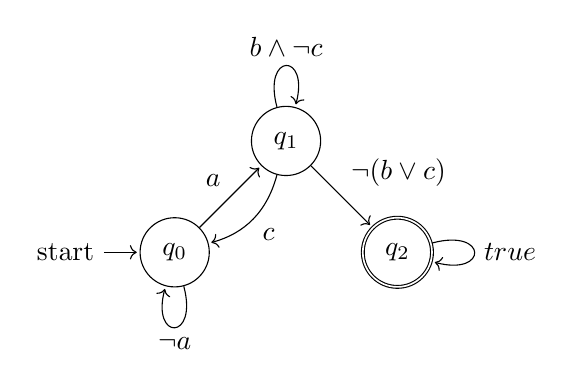
\begin{tikzpicture}[shorten >=1pt,node distance=2cm,on grid,auto] 
			\node[state,initial] (q_0)   {$q_0$}; 
			\node[state] (q_1) [above right=of q_0] {$q_1$}; 
			\node[state, accepting] (q_2) [below right=of q_1] {$q_2$}; 
			\path[->] 
			
			(q_0) edge  node {$a$} (q_1)
			edge [loop below] node {$\lnot a$} ()
			(q_1) edge  node  {$\lnot (b \lor c)$} (q_2)
			edge [bend left] node {$c$} (q_0)
			edge [loop above] node {$b \land \lnot c$} ()
			(q_2) edge [loop right] node {$true$} ();
			
		\end{tikzpicture}
		\caption{Exercise 4.1 point (a)}
		\label{fig:ex4.1:a}
		\end{figure}
	\item yes, see \autoref{fig:ex4.1:b}
	\begin{figure}[H]
		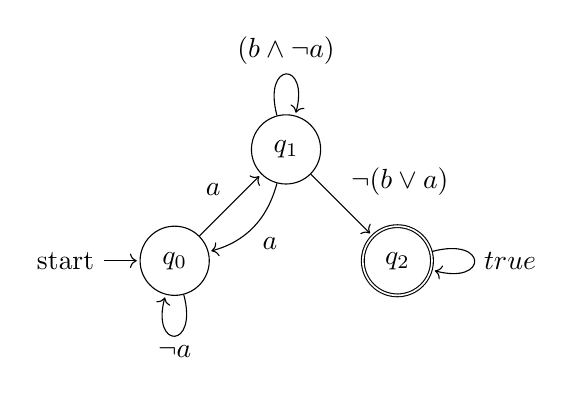
\begin{tikzpicture}[shorten >=1pt,node distance=2cm,on grid,auto] 
			\node[state,initial] (q_0)   {$q_0$}; 
			\node[state] (q_1) [above right=of q_0] {$q_1$}; 
			\node[state, accepting] (q_2) [below right=of q_1] {$q_2$}; 
			\path[->] 
			(q_0) edge  node {$a$} (q_1)
			edge [loop below] node {$\lnot a$} ()
			(q_1) edge  node  {$\lnot (b \lor a)$} (q_2)
			edge [bend left] node {$a$} (q_0)
			edge [loop above] node {$(b \land \lnot a)$} ()
			(q_2) edge [loop right] node {$true$} ();
		\end{tikzpicture}
		\caption{Exercise 4.1 point (b)}
		\label{fig:ex4.1:b}
	\end{figure}
	\item No, as $L=c^nb^{n+1}, n\ge 0$ is a subset of the property but is not a regular language. To prove it one can use the Pumping Lemma: let $P$ be the pumping length and let $w = c^Lb^{L+1}$, clearly $c^{L+x}b^{L+1}$for $x> 0$ is not in the language.
	\item Yes, see \autoref{fig:ex4.1:d} 
	\begin{figure}[H]
		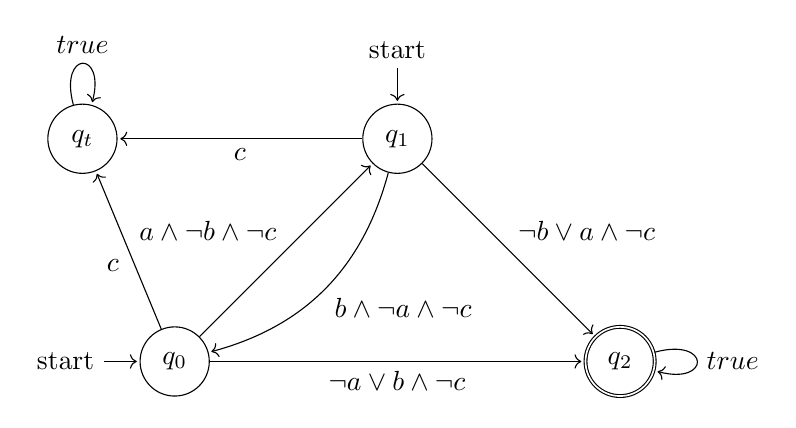
\begin{tikzpicture}[shorten >=1pt,node distance=4cm,on grid,auto] 
			\node[state,initial] (q_0)   {$q_0$}; 
			\node[state, initial above] (q_1) [above right=of q_0] {$q_1$}; 
			\node[state] (q_t) [left=of q_1] {$q_t$};
			\node[state, accepting] (q_2) [below right=of q_1] {$q_2$}; 
			\path[->] 
			(q_0) edge  node {$a \land \lnot b \land \lnot c$} (q_1)
			edge node[below] {$\lnot a \lor b \land \lnot c$} (q_2)
			edge node {$c$} (q_t)
			(q_1) edge  node  {$\lnot b \lor a \land \lnot c$} (q_2)
			edge [bend left] node {$b \land \lnot a \land \lnot c$} (q_0)
			edge node {$c$} (q_t)
			(q_2) edge [loop right] node {$true$} ()
			(q_t) edge [loop above] node {$true$} ();
		\end{tikzpicture}
		\caption{Exercise 4.1 point (b)}
		\label{fig:ex4.1:d}
	\end{figure}
	\end{enumerate}
	\subsection*{Exercise 4.2}
	\begin{enumerate}
		\item Let $n=3$ for simplicity.
		\begin{figure}[H]
			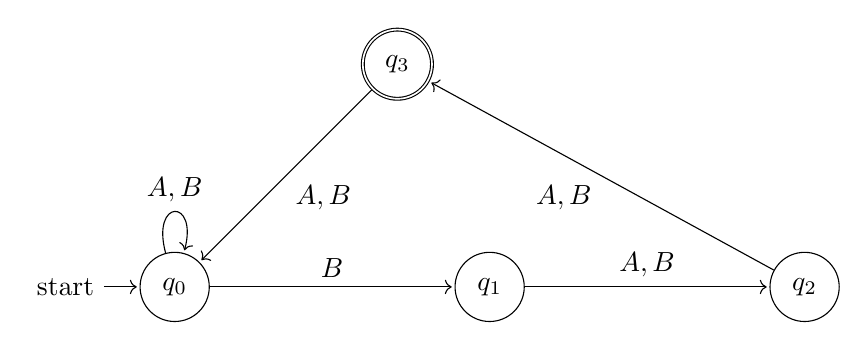
\begin{tikzpicture}[shorten >=1pt,node distance=4cm,on grid,auto] 
				\node[state, initial] (q_0) {$q_0$};
				\node[state] (q_1) [right=of q_0] {$q_1$}; 
				\node[state] (q_2)[right=of q_1] {${q_2}$};
				\node[state, accepting] (q_3) [above right=of q_0] {$q_3$}; 
				\path[->] 
				(q_0) 
				edge [loop above] node {$A,B$} ()
				edge node {$B$} (q_1)
				(q_1)
				edge node {$A, B$} (q_2)
				(q_2)
				edge node {$A,B$} (q_3)
				(q_3)
				edge node {$A,B$} (q_0);
			\end{tikzpicture}
			\caption{Exercise 4.2 point (a)}
			\label{fig:ex4.2:a}
		\end{figure}
		\item To determinize the NFA we start from $q_0$ and with a $A$ transition we can only stay in $q_0$ while using $B$ we can either move to $q_0$ or $q_1$, we call this state $q_{0,1}$.Then from this state by either $A$ or $B$ we go in the state $q_{0,2}$. Then, again by either $A$ or $B$, we go to state $q_{0,3}$ and then again to state $q_0$. See \autoref{fig:ex4.2:b}.
		\begin{figure}[H]
			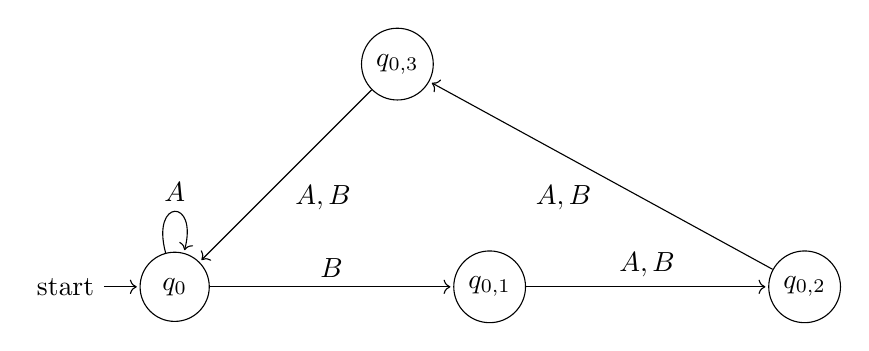
\begin{tikzpicture}[shorten >=1pt,node distance=4cm,on grid,auto] 
				\node[state, initial] (q_0) {$q_0$};
				\node[state] (q_{0,1}) [right=of q_0] {$q_{0,1}$}; 
				\node[state] (q_{0,2})[right=of q_{0,1}] {$q_{0,2}$};
				\node[state] (q_{0,3})[above right=of q_0] {$q_{0,3}$};
				\path[->] 
				(q_0) 
				edge [loop above] node {$A$} ()
				edge node {$B$} (q_{0,1})
				(q_{0,1})
				edge node {$A, B$} (q_{0,2})
				(q_{0,2})
				edge node {$A,B$} (q_{0,3})
				(q_{0,3})
				edge node {$A,B$} (q_0);
			\end{tikzpicture}
			\caption{Exercise 4.2 point (b)}
			\label{fig:ex4.2:b}
		\end{figure}
	\end{enumerate}
	\subsection*{Exercise 4.3}
	\begin{enumerate}[label=(\alph*)]
		\item \begin{enumerate}[label=(\roman*)]
			\item See \autoref{fig:ex4.3:a:i}
			\begin{figure}[H]
				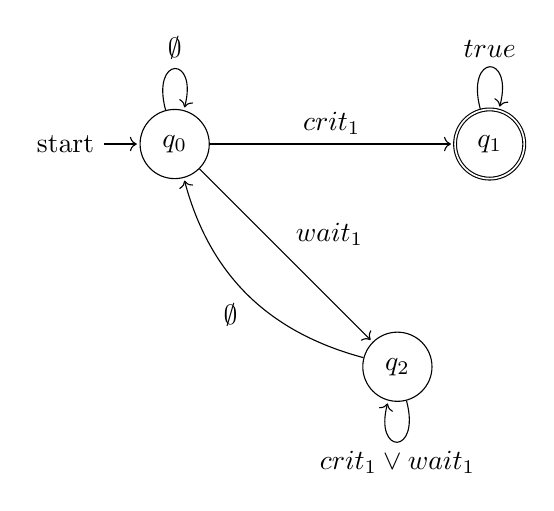
\begin{tikzpicture}[shorten >=1pt,node distance=4cm,on grid,auto] 
					\node[state, initial] (q_0) {$q_0$};
					\node[state, accepting] (q_1) [right=of q_0] {$q_1$}; 
					\node[state] (q_2)[below right=of q_0] {$q_2$};

					\path[->] 
					(q_0) 
					edge [loop above] node {$\emptyset$} ()
					edge node {$crit_1$} (q_1)
					edge node {$wait_1$} (q_2)
					(q_1)
					edge [loop above] node {$true$} ()
					(q_2)
					edge [loop below] node {$crit_1 \lor wait_1$} ()
					edge [bend left] node {$\emptyset$} (q_0);
				\end{tikzpicture}
				\caption{Exercise 4.2 point (b)}
				\label{fig:ex4.3:a:i}
			\end{figure}
			\item Recall the Semaphore based TS(\autoref{fig:semaphore-transition-system}).The product with the previous point's NFA is given in \autoref{fig:ex4.3:a:ii:ii}, as one can see no state has the right projection equal to $q_1$.
			
			\begin{figure}[H]
				\centering
				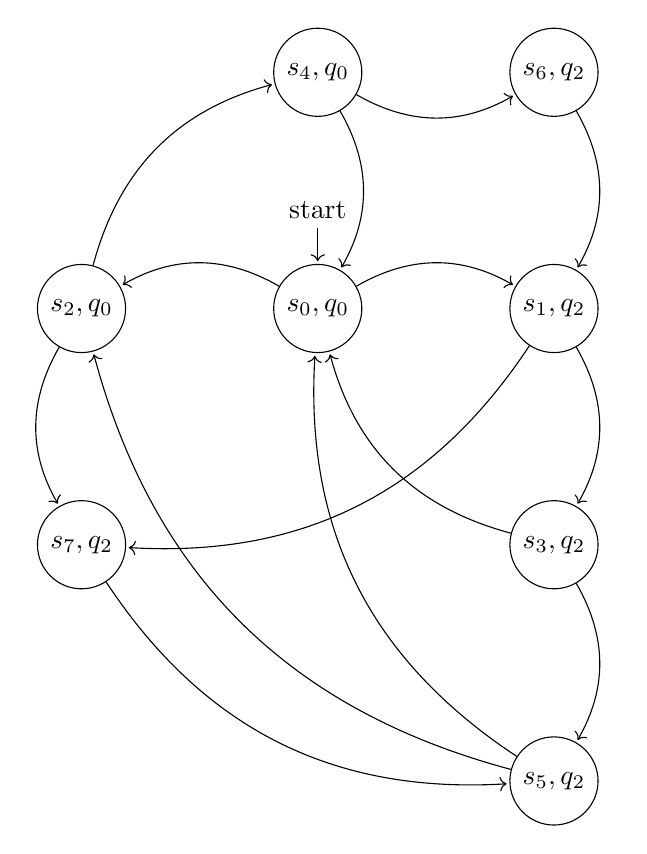
\begin{tikzpicture}[shorten >=1pt,node distance=3cm,on grid,auto] 
					\node[state, initial above] (s_0) {$s_0, q_0$};
					\node[state] (s_1) [right=of s_0] {$s_1, q_2$}; 
					\node[state] (s_2) [below=of s_1] {$s_3, q_2$};
					\node[state] (s_3) [below=of s_2] {$s_5, q_2$};
					\node[state] (s_6) [above=of s_0] {$s_4, q_0$};
					\node[state] (s_5) [left=of s_0] {$s_2, q_0$};
					\node[state] (s_4) [below=of s_5] {$s_7, q_2$};
					\node[state] (s_7) [right=of s_6] {$s_6, q_2$};
					\path[->] 
					(s_0)
					edge [bend left] node {} (s_1)
					edge [bend right] node {} (s_5)
					(s_1)
					edge [bend left] node {} (s_2)
					edge [bend left] node {} (s_4)
					(s_2)
					edge [bend left] node {} (s_3)
					edge [bend left] node {} (s_0)
					(s_3)
					edge [bend left] node {} (s_0)
					edge [bend left] node {} (s_5)
					(s_4)
					edge [bend right] node {} (s_3)
					(s_5)
					edge [bend left] node {} (s_6)
					edge [bend right] node {} (s_4)
					(s_6)
					edge [bend left] node {} (s_0)
					edge [bend right] node {} (s_7)
					(s_7)
					edge [bend left] node {} (s_1);
				\end{tikzpicture}
				\caption{Exercise 4.3. (a) point (ii): Product Graph for Semaphore Algorithm}
				\label{fig:ex4.3:a:ii:ii}
				\end{figure}
		\end{enumerate}
		\item \begin{enumerate}[label=(\roman*)]
			\item The NFA can be seen in \autoref{fig:ex4.3:b:i}.\begin{figure}[ht]
				\centering
				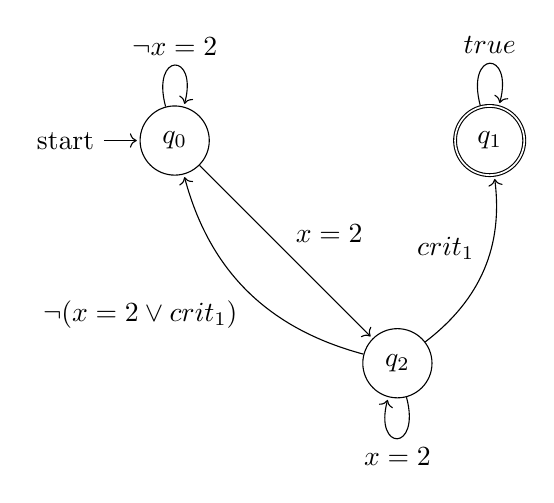
\begin{tikzpicture}[shorten >=1pt,node distance=4cm,on grid,auto] 
					\node[state, initial] (q_0) {$q_0$};
					\node[state, accepting] (q_1) [right=of q_0] {$q_1$}; 
					\node[state] (q_2)[below right=of q_0] {$q_2$};
					
					\path[->] 
					(q_0) 
					edge [loop above] node {$\lnot x=2$} ()
					edge node {$x=2$} (q_2)
					(q_1)
					edge [loop above] node {$true$} ()
					(q_2)
					edge [loop below] node {$x=2$} ()
					edge [bend right] node {$crit_1$} (q_1)
					edge [bend left] node {$\lnot (x=2 \lor crit_1)$} (q_0);
				\end{tikzpicture}
				\caption{Exercise 4.3 point (b) the NFA of Bad Prefixes for "process 1 never enters its critical section from a state with x=2"}
				\label{fig:ex4.3:b:i}
			\end{figure}
			\item Recall Peterson's TS in \autoref{fig:peterson-transition-system} and then we show (part of) the product graph in \autoref{fig:ex4.3:b:ii:ii}
			\begin{figure}[H]
				\centering
				\begin{tikzpicture}[shorten >=1pt,node distance=3cm,on grid,auto] 
					\node[state, initial] (s_0) {$s_0, q_0$};
					\node[state, initial] (s_1) [right =of s_0] {$s_1, q_2$};
					\node[state] (s_2) [below=of s_0] {$s_2, q_2$};
					\node[state] (s_3) [below=of s_2] {$s_6, q_1$};
					\path[->] 
					(s_0)
					edge [bend left] node {} (s_2)
					(s_2)
					edge [bend left] node {} (s_3);
				\end{tikzpicture}
				\caption{Exercise 4.3 point (b) (ii) part of the product automata for the property "process 1 never enters its critical section from a state with x=2". Clearly we can reach a state $s$ where $L(s)=q_1$. So we conclude the TS does not satisfy the property.}
				\label{fig:ex4.3:b:ii:ii}
			\end{figure}
		\end{enumerate}
	\end{enumerate}
	\subsection*{Exercise 4.4}
	\begin{enumerate}[label=(\alph*)]
		\item It is true. Take the NFA $N=(Q, \Sigma, \delta, Q_0, F)$ corresponding to $\mathcal{L}$, then by hypothesis this NFA accepts the minimal bad prefixes of $P_{safe}$ and some other bad prefixes. It is enough to remove any outgoing edge from end states in $N$, obtaining the NFA $N'$, to get an NFA accepting the minimal bad prefixes of $P_{safe}$. If $w$($|w|=n$) is a minimal bad prefix then it is accepted by $N$ by construction, which means there exists a run $\pi$ such that $\exists i. \pi_i \in F$ and $\pi_1 \rightarrow^{w_1} \pi_2 \rightarrow^{w_2} ... \rightarrow^{w_n} \pi_i$.
		Then it is obvious that there cannot be another $j$ such that $j<i$ and $\pi_j\in F$ because this would mean $w'=w_1...w_j$ is a bad prefix (since $L \subseteq BadPref(P_{safe})$) of a minimal bad prefix $w$.
		Then we know that $N'$ can imitate this same path and thus accept any minimal bad prefix of $P_{safe}$. For the other direction, namely that $N'$ accepts only the (minimal) bad prefixes: since $N'$ is $N$ after we remove some edges it cannot expand the language accepted, thus $N'$ accepts only Bad Prefixes of $L_{safe}$ and because no end state has outgoing transition it accepts only the minimal ones.
		\item False. Consider the regular safety property $\emptyset$, then $MinBadPref(P_{safe})=\emptyset$ and $BadPref(P_{safe})=(2^{\{0,1\}})^{\omega}$. Now consider $L=\{\{0\}^n\{1\}^n+1| \forall n \ge 0\}$ which is clearly not regular.
	\end{enumerate}
	\subsection*{Exercise 4.5}
	First, some considerations on the NFA: it is described by the RE: $$((bc)^*a.(a^*.(b+ab).a^*.(b+ab))^*.c)^*.(bc)^*a.c$$.
	One possible way to describe the bad prefixes represented by this NFA could be: $c \in A_i \implies A_{i-1}= \{a\}$.
	\begin{figure}[H]
		\centering
		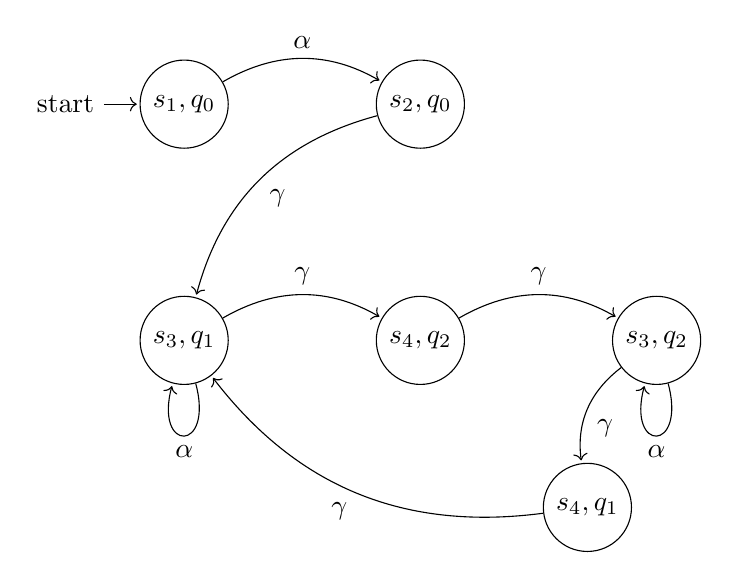
\begin{tikzpicture}[shorten >=1pt,node distance=3cm,on grid,auto] 
			\node[state, initial] (s_0) {$s_1, q_0$};
			\node[state] (s_1) [right=of s_0] {$s_2, q_0$};
			\node[state] (s_2) [below=of s_0] {$s_3, q_1$};
			\node[state] (s_3) [right=of s_2] {$s_4, q_2$};
			\node[state] (s_4) [right=of s_3] {$s_3, q_2$};
			\node[state] (s_5) [below right=of s_3] {$s_4, q_1$};
			\path[->] 
			(s_0)
			edge [bend left] node {$\alpha$} (s_1)
			(s_1)
			edge [bend right] node {$\gamma$} (s_2)
			(s_2)
			edge [loop below] node {$\alpha$} ()
			edge [bend left] node {$\gamma$} (s_3)
			(s_3)
			edge [bend left] node {$\gamma$} (s_4)
			(s_4)
			edge [loop below] node {$\alpha$} ()
			edge [bend right] node {$\gamma$} (s_5)
			(s_5)
			edge [bend left] node {$\gamma$} (s_2);
		\end{tikzpicture}
		\caption{Exercise 4.5, the reachable fragment of the product $TS \otimes A$}
		\label{fig:ex4.5}
	\end{figure}
	\subsection*{Exercise 4.6}
	I read this property as "Always, if $a$ becomes valid and $b \land \lnot c$ holds in one of the states \textit{before} then in every state \textit{after} neither $a$ nor $b$ hold until a $c$ holds". I consider the set $AP=\{a,b, c\}$.
	\begin{enumerate}[label=(\alph*)]
		\item See \autoref{fig:ex4.1:a}. 
		\begin{figure}[H]
			\centering
			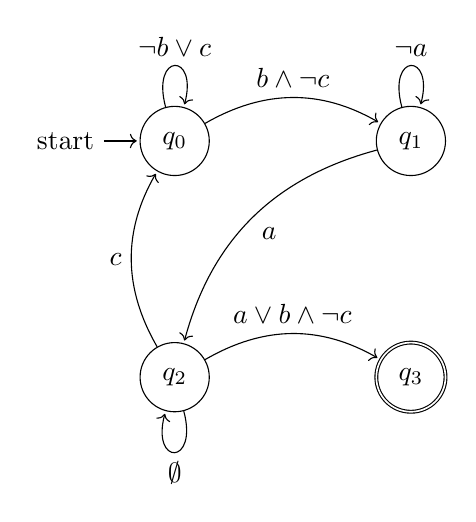
\begin{tikzpicture}[shorten >=1pt,node distance=3cm,on grid,auto] 
				\node[state, initial] (q_0) {$q_0$};
				\node[state] (q_1) [right=of q_0] {$q_1$};
				\node[state] (q_2) [below=of q_0] {$q_2$};
				\node[state, accepting] (q_3) [right=of q_2] {$q_3$};
				\path[->] 
				(q_0)
				edge [bend left] node {$b \land \lnot c$} (q_1)
				edge [loop above] node {$\lnot b \lor c$} ()
				(q_1)
				edge [loop above] node {$\lnot a$} ()
				edge [bend right] node {$a$} (q_2)
				(q_2)
				edge [loop below] node {$\emptyset$} () 
				edge [bend left] node {$a \lor b \land \lnot c$} (q_3)
				edge [bend left] node {$c$} (q_0);
				\end{tikzpicture}
			\caption{Exercise 4.6 part (a): The NFA $A$ accepting $\text{MinBadPref}(P_{safe})$}
			\label{fig:ex4.6:a}
		\end{figure}
		\item The TS satisfies the property as a state of the form $x, q_3$ is not reachable, see \autoref{fig:ex4.6:b}. \begin{figure}[H]
			\centering
			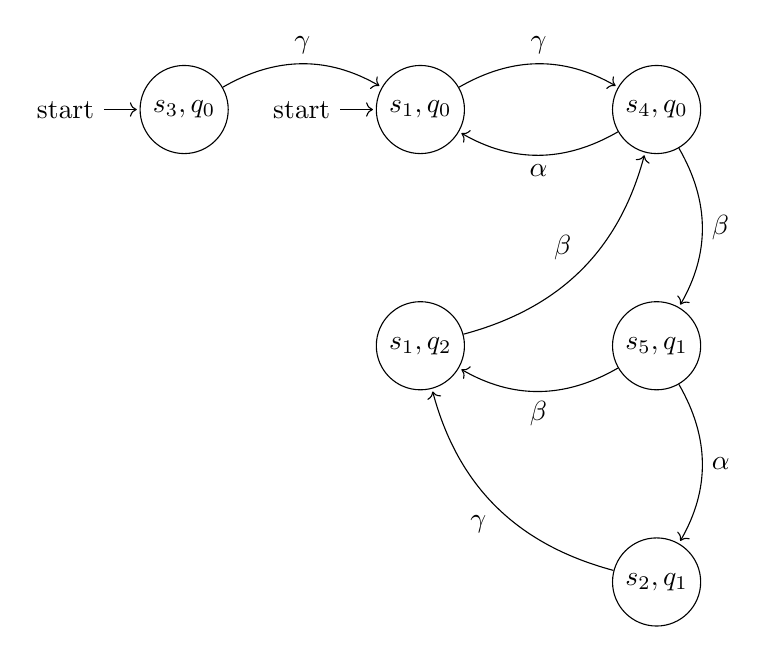
\begin{tikzpicture}[shorten >=1pt,node distance=3cm,on grid,auto] 
				\node[state, initial] (s_0) {$s_3, q_0$};
				\node[state, initial] (s_1)[right=of s_0] {$s_1, q_0$};
				\node[state] (s_2) [right=of s_1] {$s_4, q_0$};
				\node[state] (s_4) [below=of s_1] {$s_1, q_2$};
				\node[state] (s_3) [right=of s_4] {$s_5, q_1$};
				\node[state] (s_5) [below=of s_3] {$s_2, q_1$};
				\path[->] 
				(s_0)
				edge [bend left] node {$\gamma$} (s_1)
				(s_1)
				edge [bend left] node {$\gamma$} (s_2)
				(s_2)
				edge [bend left] node {$\alpha$} (s_1)
				edge [bend left] node {$\beta$} (s_3)
				(s_3)
				edge [bend left] node {$\alpha$} (s_5)
				edge [bend left] node {$\beta$} (s_4)
				(s_4)
				edge [bend right] node {$\beta$} (s_2)
				(s_5)
				edge [bend left] node {$\gamma$} (s_4);
			\end{tikzpicture}
			\caption{Exercise 4.6 part (b): The Product $TS \otimes A$}
			\label{fig:ex4.6:b}
		\end{figure}
	\end{enumerate}
	\subsection*{Exercise 4.7}
	\begin{enumerate}[label=(\alph*)]
		\item True. $$\underbrace{L(E_1.F^\omega + E_2.F^\omega)}_{L1} = \underbrace{L(E_1).L(F)^\omega}_{L2} \cup \underbrace{L(E_2).L(F)^\omega}_{L3} $$
		so any word $w \in L1$ is either a word in $L2$ or $L3$ (non exclusive or). 
		$$
		\underbrace{L((E_1+E_2).F^\omega)}_{L4} =
		\underbrace{L(E_1+E_2).L(F)^\omega}_{L5}
		$$
		Suppose, without loss of generality, $w \in L2$, then it is made of a prefix $p$ in $L(E_1)$ and an $\omega$-suffix $s$ in $L(F)^\omega$. Since $p \in L(E_1) \implies p \in L(E_1+E_2)$ we conclude. For the other direction: if $w \in L4$ then it is made of a prefix $p$ in $L(E_1 + E_2)$ and a suffix in $L(F^\omega)$, since $p \in L(E_1)$ or $p \in L(E_2)$ we conclude. 
		\item False. Take $\Sigma=\{a,b,c\}$ as an alphabet, $E=a, F_1=b, F_2=c$. Then $a.(a.b)^\omega \in L(E).(F_1+F_2)^\omega$ by definition of the $\omega$ operator. But $L(E.F^\omega_1)+L(E.F^\omega_2)=\{a.(b)^\omega, a.(c)^\omega\}$
		\item True. We can just show $$\underbrace{L(F.F^*)^\omega}_{L1}=\underbrace{L(F)^\omega}_{L2}$$ Take any word $w \in L1$. $w$, is by definition, an infinite concatenation of words $w_i \in F.F^*$. We prove that there exists a word $w'\in L2$ such that $\forall i \in \mathbb{N}. w_1...w_i$ is a prefix of $w'$. This equals to say that $w'=w$. By induction:
		\begin{itemize}
			\item i=1: by definition $w_1$ is a concatenation of one or more (finite) words from $F$, i.e. $w_1=w_{1,1}.w_{1,2}\dots w_{1,n}$. Let $w'_1=w_{1,1}, w'_2=w_{1,2}\dots w'_n=w_{1,n}$.
			\item i=k+1: suppose, by inductive hypothesis, that the prefix $w_1...w_k$ is long $q$. suppose $w_{k+1}=w_{k+1,1}.w_{k+1,2}\dots w_{k+1,t}$ then let $w'_{q+1}=w_{k+1,1}, w'_{q+2}=w_{k+1,2}\dots w'_{q+t}=w_{k+1,t}$.
		\end{itemize}
		For the other direction, namely that $w \in L2 \implies w \in L1$ we note that $L(F)\subseteq L(F.F^*) \implies L(F)^\omega \subseteq L(F.F^*)^\omega$.
		\item False. Take $\Sigma=\{a,b\}$ as an alphabet, $E=a, F=b$. Then $a.(a.b)^\omega \in L(E^*.F)^\omega$ but there is no word with infinite $a$s in $E^*.F^\omega$ as the $\omega$ operator is applied only to the language $\{b\}$.
	\end{enumerate}
	\subsection*{Exercise 4.8}
	We need to proceed by cases on the form of $G$, let $F$ be an operator which takes in input a generalized $\omega$-regular expression and returns one equivalent of the form $E+E_1.F_1^\omega+\dots E_n.F^\omega_n$:
	\begin{enumerate}
		\item $F(\emptyset)=\emptyset$
		\item $F(\epsilon)=\epsilon$
		\item $F(A)=\{A\}$
		\item $F(G_1+G_2)=F(G_1)+F(G_2)$
		\item $F(G_1.G_2)$: we know by inductive hypothesis that $F(G_1)=E+E_1.F^\omega_1+\dots E_n.F_n^\omega$ and $F(G_2)=E'+E'_1.(F_1')^\omega+\dots E'_t.(F_t')^\omega$ then we need to concatenate finite words of $G_1$ with finite and infinite words of $G_2$ and append the infinite words of $G_1$:
		$$
		F(G_1.G_2)=E.E'+E_1.F^\omega_1+\dots E_n.F_n^\omega+E.E'_1.(F_1')^\omega+\dots E.E'_t.(F_t')^\omega
		$$
		\item $F(G^*)$: by inductive hypothesis $F(G)=E+E_1.F^\omega_1+\dots E_n.F_n^\omega$ thus $$F(G^*)=E^*+E^*.E_1.F^\omega_1+\dots E^*.E_n.F_n^\omega$$
		\item $F(G^\omega)$: by inductive hypothesis $F(G)=E+E_1.F^\omega_1+\dots E_n.F_n^\omega$. Following the same reasoning as for the Kleene closure, $F(G^\omega)=(E \setminus \epsilon)^\omega$.
	\end{enumerate}
	\subsection*{Exercise 4.9}
	\begin{figure}[H]
		\centering
		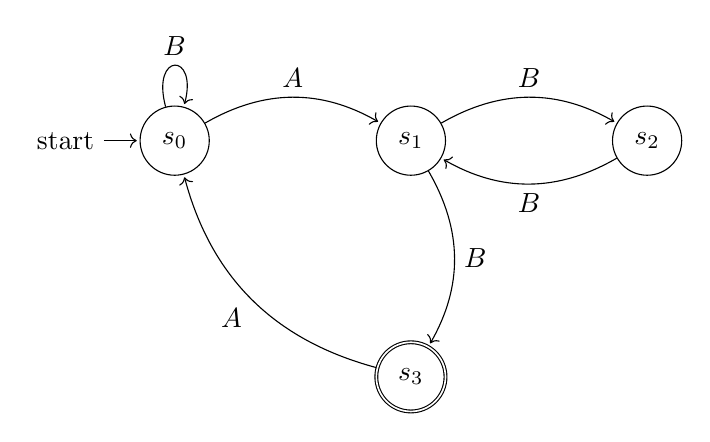
\begin{tikzpicture}[shorten >=1pt,node distance=3cm,on grid,auto] 
			\node[state, initial] (s_0) {$s_0$};
			\node[state] (s_1)[right=of s_0] {$s_1$};
			\node[state] (s_2) [right=of s_1] {$s_2$};
			\node[state, accepting] (s_3) [below=of s_1] {$s_3$};
			\path[->] 
			(s_0)
			edge [bend left] node {$A$} (s_1)
			edge [loop above] node {$B$} ()
			(s_1)
			edge [bend left] node {$B$} (s_2)
			edge [bend left] node {$B$} (s_3)
			(s_2)
			edge [bend left] node {$B$} (s_1)
			(s_3)
			edge [bend left] node {$A$} (s_0);
		\end{tikzpicture}
		\caption{Exercise 4.9. NBA for the property "infinitely many A, and between two A there is an odd number of B"}
		\label{fig:ex4.9}
	\end{figure}
	\subsection*{Exercise 4.10}
	\begin{enumerate}[label=(\alph*)]
		\item See \autoref{fig:ex4.10:a} for a visual description of the NBA. An $\omega$-regular expression is: $(B+C)^*.(A.((B.B)^*.B+(C.C)^*.C))^\omega$ 
		\begin{figure} \centering
			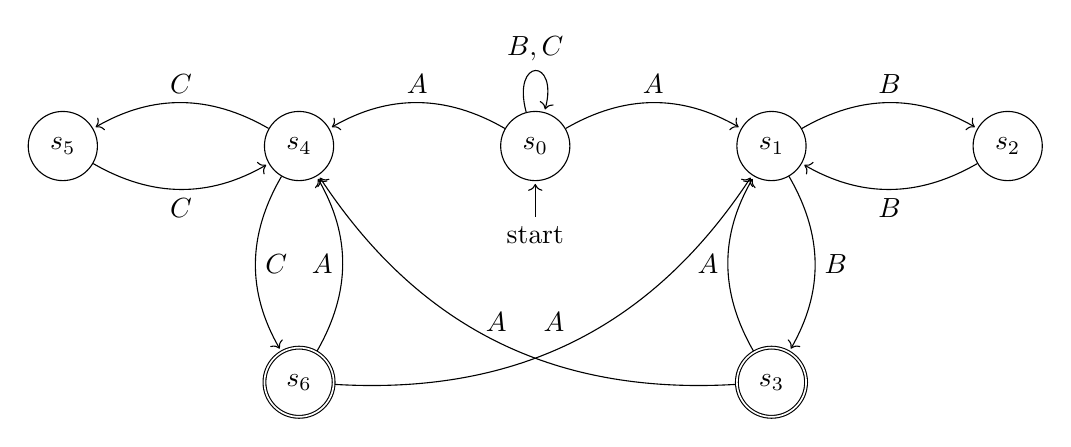
\begin{tikzpicture}[shorten >=1pt,node distance=3cm,on grid,auto] 
				\node[state, initial below] (s_0) {$s_0$};
				\node[state] (s_1)[right=of s_0] {$s_1$};
				\node[state] (s_2) [right=of s_1] {$s_2$};
				\node[state, accepting] (s_3) [below=of s_1] {$s_3$};
				\node[state] (s_4) [left=of s_0] {$s_4$};
				\node[state] (s_5) [left=of s_4] {$s_5$};
				\node[state, accepting] (s_6) [below=of s_4] {$s_6$};
				\path[->] 
				(s_0)
				edge [bend left] node {$A$} (s_1)
				edge [loop above] node {$B,C$} ()
				edge [bend right] node[above] {$A$} (s_4)
				(s_1)
				edge [bend left] node {$B$} (s_2)
				edge [bend left] node {$B$} (s_3)
				(s_2)
				edge [bend left] node {$B$} (s_1)
				(s_3)
				edge [bend left] node[above] {$A$} (s_4)
				edge [bend left] node {$A$} (s_1)
				(s_4)
				edge [bend right] node[above] {$C$} (s_5)
				edge [bend right] node {$C$} (s_6)
				(s_5)
				edge [bend right] node[below] {$C$} (s_4)
				(s_6)
				edge [bend right] node {$A$} (s_4)
				edge [bend right] node {$A$} (s_1);
			\end{tikzpicture}
			\caption{Exercise 4.10 NBA for point (c)}
			\label{fig:ex4.10:a}
		\end{figure}
		\item See the NBA in \autoref{fig:ex4.10:b}, the $\omega$-regular expression becomes $$((B+C)^*.(A.((B.B)^*.B+(C.C)^*.C))).(A.((B.B)^*.B))^\omega$$ \begin{figure} 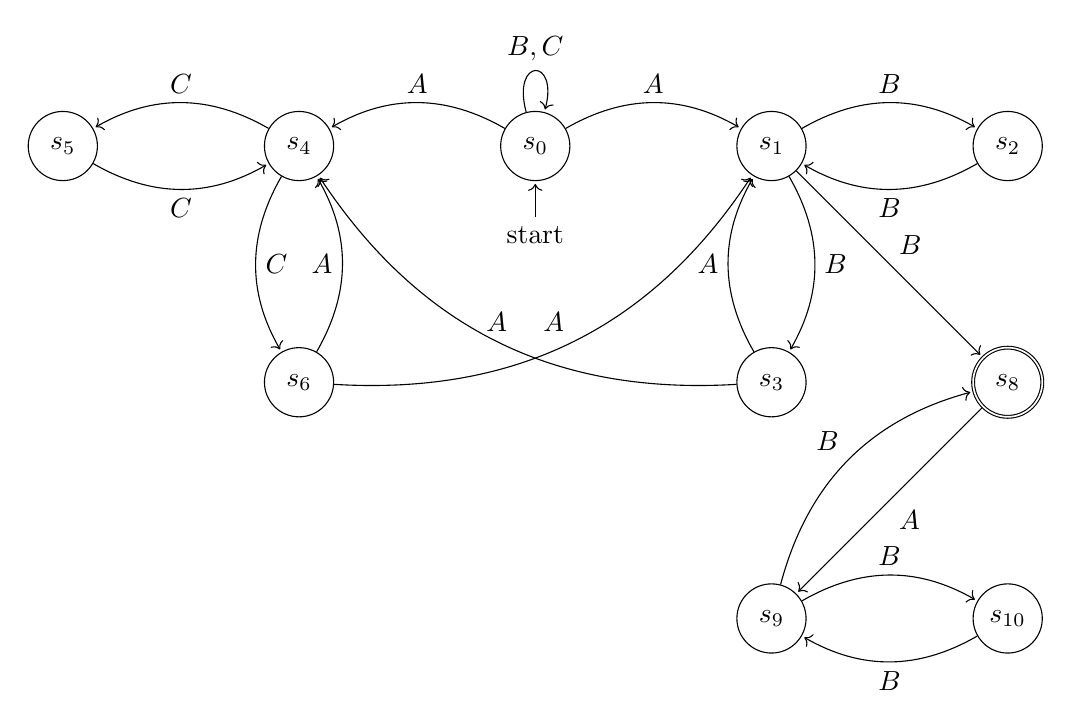
\begin{tikzpicture}[shorten >=1pt,node distance=3cm,on grid,auto] 
			\node[state, initial below] (s_0) {$s_0$};
			\node[state] (s_1)[right=of s_0] {$s_1$};
			\node[state] (s_2) [right=of s_1] {$s_2$};
			\node[state] (s_3) [below=of s_1] {$s_3$};
			\node[state] (s_4) [left=of s_0] {$s_4$};
			\node[state] (s_5) [left=of s_4] {$s_5$};
			\node[state] (s_6) [below=of s_4] {$s_6$};
			\node[state, accepting] (s_8) [below=of s_2] {$s_8$};
			\node[state] (s_9) [below=of s_3] {$s_9$};
			\node[state] (s_{10}) [right=of s_9] {$s_{10}$};
			\path[->] 
			(s_0)
			edge [bend left] node {$A$} (s_1)
			edge [loop above] node {$B,C$} ()
			edge [bend right] node[above] {$A$} (s_4)
			(s_1)
			edge [bend left] node {$B$} (s_2)
			edge [bend left] node {$B$} (s_3)
			edge node {$B$} (s_8)
			(s_2)
			edge [bend left] node {$B$} (s_1)
			(s_3)
			edge [bend left] node[above] {$A$} (s_4)
			edge [bend left] node {$A$} (s_1)
			(s_4)
			edge [bend right] node[above] {$C$} (s_5)
			edge [bend right] node {$C$} (s_6)
			(s_5)
			edge [bend right] node[below] {$C$} (s_4)
			(s_6)
			edge [bend right] node {$A$} (s_4)
			edge [bend right] node {$A$} (s_1)
			(s_8)
			edge node {$A$} (s_9)
			(s_9)
			edge [bend left] node {$B$} (s_{10})
			edge [bend left] node {$B$} (s_8)
			(s_{10})
			edge [bend left] node {$B$} (s_9);
		\end{tikzpicture}
		\caption{Exercise 4.10 NBA for point (b)}
		\label{fig:ex4.10:b}
		\end{figure}
	 	\item \begin{figure} \centering
	 		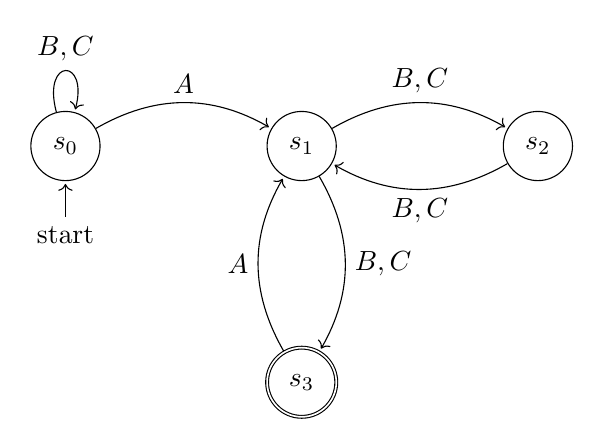
\begin{tikzpicture}[shorten >=1pt,node distance=3cm,on grid,auto] 
	 			\node[state, initial below] (s_0) {$s_0$};
	 			\node[state] (s_1)[right=of s_0] {$s_1$};
	 			\node[state] (s_2) [right=of s_1] {$s_2$};
	 			\node[state, accepting] (s_3) [below=of s_1] {$s_3$};
	 			\path[->] 
	 			(s_0)
	 			edge [bend left] node {$A$} (s_1)
	 			edge [loop above] node {$B,C$} ()
	 			(s_1)
	 			edge [bend left] node {$B,C$} (s_2)
	 			edge [bend left] node {$B,C$} (s_3)
	 			(s_2)
	 			edge [bend left] node {$B,C$} (s_1)
	 			(s_3)
	 			edge [bend left] node {$A$} (s_1);
	 		\end{tikzpicture}
	 		\caption{Exercise 4.10 NBA for point (c)}
	 		\label{fig:ex4.10:c}
	 	\end{figure}
	 	\item \begin{figure} \centering
	 		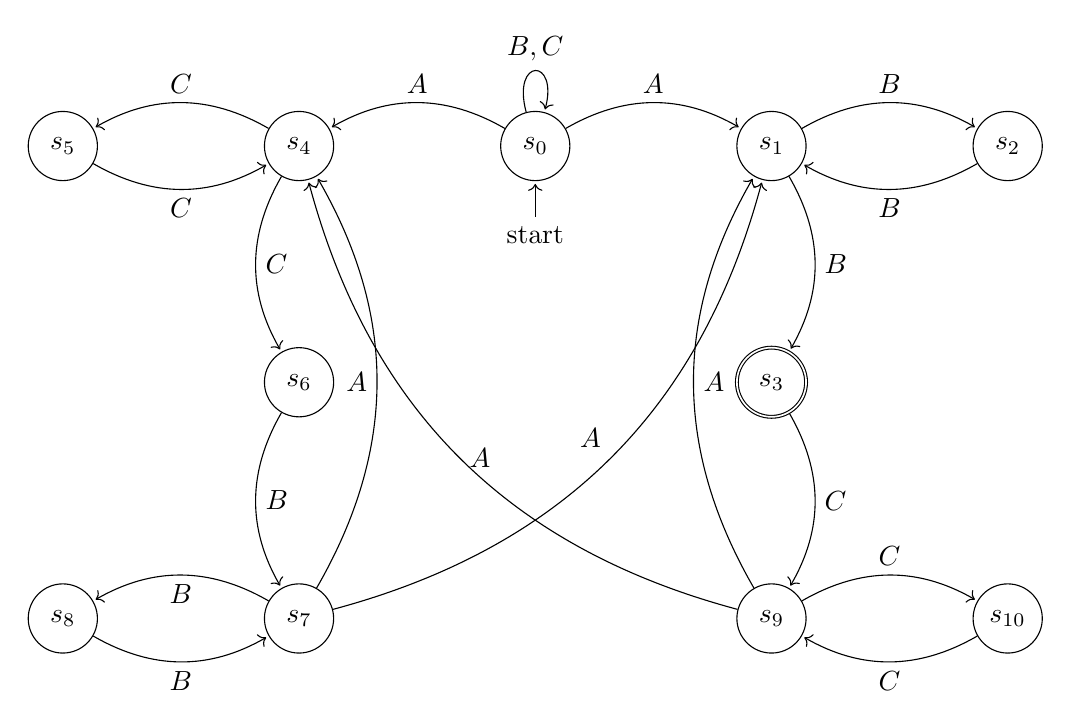
\begin{tikzpicture}[shorten >=1pt,node distance=3cm,on grid,auto] 
	 			\node[state, initial below] (s_0) {$s_0$};
	 			\node[state] (s_1)[right=of s_0] {$s_1$};
	 			\node[state] (s_2) [right=of s_1] {$s_2$};
	 			\node[state, accepting] (s_3) [below=of s_1] {$s_3$};
	 			\node[state] (s_4) [left=of s_0] {$s_4$};
	 			\node[state] (s_5) [left=of s_4] {$s_5$};
	 			\node[state] (s_6) [below=of s_4] {$s_6$};
	 			% New nodes mirroring s1,s2,s3
	 			\node[state] (s_7) [below=of s_6] {$s_7$};
	 			\node[state] (s_8) [left=of s_7] {$s_8$};
	 			% New nodes mirroring s4,s5,s6
	 			\node[state] (s_9) [below=of s_3] {$s_9$};
	 			\node[state] (s_{10}) [right=of s_9] {$s_{10}$};
	 			\path[->] 
	 			(s_0)
	 			edge [bend left] node {$A$} (s_1)
	 			edge [loop above] node {$B,C$} ()
	 			edge [bend right] node[above] {$A$} (s_4)
	 			(s_1)
	 			edge [bend left] node {$B$} (s_2)
	 			edge [bend left] node {$B$} (s_3)
	 			(s_2)
	 			edge [bend left] node {$B$} (s_1)
	 			(s_3)
	 			edge [bend left] node {$C$} (s_9)
	 			(s_4)
	 			edge [bend right] node[above] {$C$} (s_5)
	 			edge [bend right] node {$C$} (s_6)
	 			(s_5)
	 			edge [bend right] node[below] {$C$} (s_4)
	 			(s_6)
	 			edge [bend right] node {$B$} (s_7)
	 			% New triplet behaving like s4-s5-s6
	 			(s_7)
	 			edge [bend right] node {$A$} (s_1)
	 			edge [bend right] node {$A$} (s_4)
	 			edge [bend right] node {$B$} (s_8)
	 			(s_8)
	 			edge [bend right] node[below] {$B$} (s_7)
	 			(s_9)
	 			edge [bend left] node[right] {$A$} (s_4)
	 			edge [bend left] node[right] {$A$} (s_1)
	 			edge [bend left] node {$C$} (s_{10})
	 			(s_{10})
	 			edge [bend left] node {$C$} (s_9);
	 		\end{tikzpicture}
	 		\caption{Exercise 4.10 NBA for point (d)}
	 		\label{fig:ex4.10:d}
	 	\end{figure}
	\end{enumerate}
	\subsection*{Exercise 4.11}
	The Automata has two initial states and two final states and it is depicted in \autoref{fig:ex4.11}.
	\begin{figure}[H] \centering
		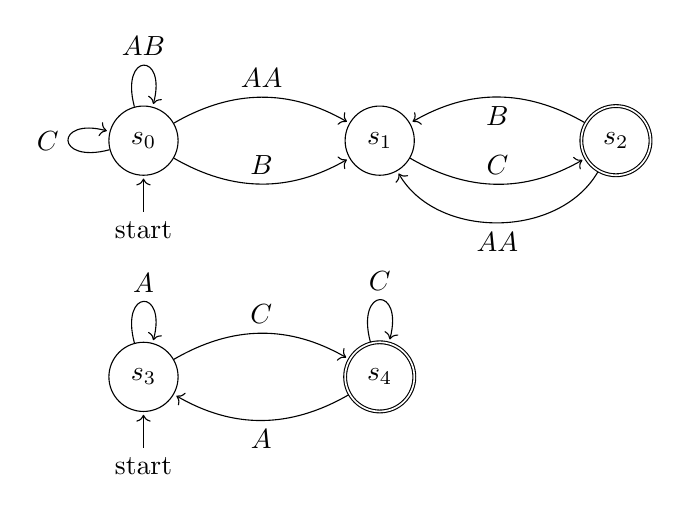
\begin{tikzpicture}[shorten >=1pt,node distance=3cm,on grid,auto] 
			\node[state, initial below] (s_0) {$s_0$};
			\node[state] (s_1)[right=of s_0] {$s_1$};
			\node[state, accepting] (s_2)[right=of s_1] {$s_2$};
			\node[state, initial below] (s_3)[below=of s_0] {$s_3$};
			\node[state, accepting] (s_4) [right=of s_3] {$s_4$};
			\path[->] 
			(s_0)
			edge [loop above] node {$AB$} ()
			edge [loop left] node {$C$} () 
			edge [bend left] node {$AA$} (s_1)
			edge [bend right] node {$B$} (s_1)
 			(s_1)
			edge [bend right] node {$C$} (s_2)
			(s_2)
			edge [bend left=60] node {$AA$} (s_1)
			edge [bend right] node {$B$} (s_1)
			(s_3)
			edge [loop above] node {$A$} ()
			edge [bend left] node {$C$} (s_4)
			(s_4)
			edge [loop above] node {$C$} ()
			edge [bend left] node {$A$} (s_3);
		\end{tikzpicture}
		\caption{Exercise 4.11 NBA for the $\omega$-regular expression $(AB+C)^*((AA+B)C)^\omega+(A^*C)^\omega$}
		\label{fig:ex4.11}
	\end{figure}
	\newpage
	\subsection{Appendix}
		\begin{figure}[H]
		\centering    
		\adjustbox{scale=0.8,center}{
			\begin{tikzcd}
				&  & {s_0:\; req_1, req_2, x=1} \arrow[d] \arrow[rrrd] &  &  & {s_1:\; req_1, req_2, x=2} \arrow[d] \arrow[llld] &  &                                                       \\
				{s_6: crit_1, req_2,  x=2} \arrow[rrrrru] \arrow[rrddd] &  & {s_2:\; wait_1, req_2, x=2} \arrow[d] \arrow[ll]  &  &  & {s_3:\; req_1, wait_2, x=1} \arrow[d] \arrow[rr]  &  & {s7: req_1, crit_2, x=1} \arrow[lllllu] \arrow[llddd] \\
				&  & {s_4:\; wait_1, wait_2, x=1} \arrow[dd]           &  &  & {s_5:\; wait_1, wait_2, x=2} \arrow[dd]           &  &                                                       \\
				&  &                                                   &  &  &                                                   &  &                                                       \\
				&  & {s_8:\; crit_1, wait_2, x=1} \arrow[rrruuu]       &  &  & {s_9:\; wait_1, crit_2, x=2} \arrow[llluuu]       &  &                                                      
			\end{tikzcd}
		}
		\caption{Transition Graph for Peterson Algorithm, $TS_{pet}$}
		\label{fig:peterson-transition-system}
	\end{figure}
	\begin{figure}[H]
		\centering    
		\adjustbox{scale=1,center}{
			\begin{tikzcd}
				&& {s_0:\; req_1, req_2} \\
				& {s_1:\; wait_1, req_2} && {s_2:\; req_1, wait_2} \\
				& {s_3:\; crit_1, req_2} && {s_4:\; req_1, crit_2} \\
				{s_5:\; crit_1, wait_2} &&&& {s_6:\; wait_1, crit_2} \\
				&& {s_7:\; wait_1, wait_2}
				\arrow[from=1-3, to=2-2]
				\arrow[from=1-3, to=2-4]
				\arrow[from=2-2, to=3-2]
				\arrow[from=2-2, to=5-3]
				\arrow[from=2-4, to=3-4]
				\arrow[from=2-4, to=5-3]
				\arrow[from=3-2, to=1-3]
				\arrow[from=3-2, to=4-1]
				\arrow[from=3-4, to=1-3]
				\arrow[from=3-4, to=4-5]
				\arrow[from=4-1, to=2-4]
				\arrow[from=4-5, to=2-2]
				\arrow[from=5-3, to=4-1]
				\arrow[from=5-3, to=4-5]
			\end{tikzcd}
		}
		\caption{Transition Graph for Semaphore Algorithm, $TS_{sem}$}
		\label{fig:semaphore-transition-system}
	\end{figure}
\end{document}
